%%%%%%%%%%%%%%%%%%%%%%%%%%%%%%%%%%%%%%%%%%%%%%%%%%%
%% P3: Phenomenology of Particle Physics                         
%%
%% Author:  André Rubbia                   		 
%%
%% Figure 2.23 Sketch for the calculation of the energy transferred to an atomic electron by a heavy charged particle.
%%
%% This work is licensed under the Creative Commons Attribution 4.0 International License. 
%% To view a copy of this license, visit http://creativecommons.org/licenses/by/4.0/ or 
%% send a letter to Creative Commons, PO Box 1866, Mountain View, CA 94042, USA.
%%
%%
%%%%%%%%%%%%%%%%%%%%%%%%%%%%%%%%%%%%%%%%%%%%%%%%%%%

\documentclass[a4paper,10pt]{article}

\usepackage[T1]{fontenc}
\usepackage[utf8]{inputenc}
\usepackage{lmodern}
\usepackage[labelfont=bf]{caption}
\usepackage{upgreek}
\usepackage{amssymb}
\usepackage{amsmath}

\usepackage{tikz}
\usepackage{pgfplots}
\pgfplotsset{compat=1.17}
\usepgfplotslibrary{ternary}
\usepgfplotslibrary{fillbetween}
\usepgfplotslibrary{external}


\def\d{\mathrm{d}}

\begin{document}

%%%%%%%%%%%%%%%   FIGURE  %%%%%%%%%%%%%%%%%%%%%%%%%%%%%%
\begin{figure}[htb]
\begin{center}
    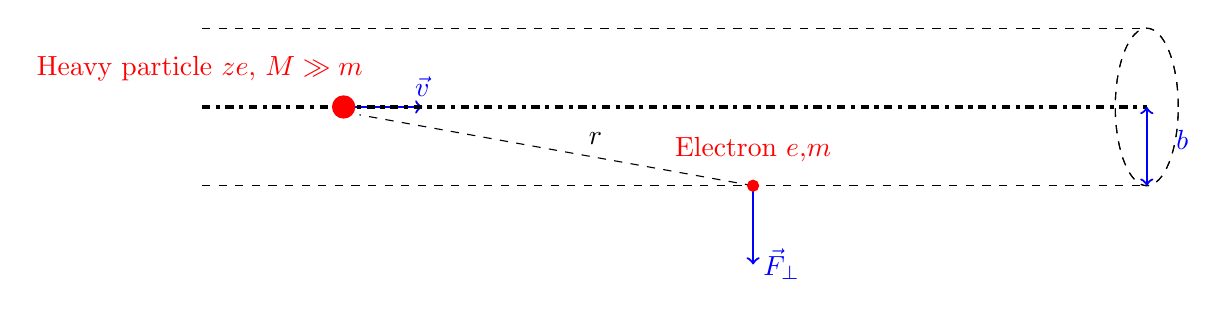
\begin{tikzpicture}[scale=1]
         \draw[dashed] (-7,0) -- (5,0);
         \draw[dashed] (-7,2) -- (5,2);
         \draw[dashed] (0,0) -- (-5,0.9);
         \draw[dashed]  (5,1) ellipse (0.4 and 1);
          \draw[dashed]  (5,1) ellipse (0.4 and 1);
        \draw[blue,thick,->] (-5.2,1) -- +(0:1) node[above] {$\vec v$};
         \draw[blue,thick,->] (0,0) -- +(-90:1) node[right] {$\vec F_\perp$};
         \draw[line width=1.5, dash dot] (-7,1) -- (5,1);
         \filldraw [red] (0,0) circle (2pt) node[above=5pt] {Electron $e$,$m$};
         \filldraw [red] (-5.2,1) circle (4pt) node[above=6pt, xshift=-52pt] {Heavy particle $ze$, $M\gg m$};
         \draw[thick,blue,<->] (5,0) -- (5,1) node[right=7pt, yshift=-12pt] {$b$};
        \node at (-2.,0.6) {$r$};
  \end{tikzpicture}
\caption{Sketch for the calculation of the energy transferred to an atomic electron by a heavy charged particle.}
\end{center}
\end{figure}
%%%%%%%%%%%%%%%   END FIGURE  %%%%%%%%%%%%%%%%%%%%%%%%%%%%%%
\end{document}
